\chapter{Ground Vibration Test Frequency Response Plots}
\label{ap:gvtPlot}

The plots each indicate the acceleration response at a location to an impulse input at a location. The locations are labeled by node number and direction. The locations of the respective nodes can be found in Figure \ref{fig:accelPlacement}.

\begin{figure}[H]
    \centering
    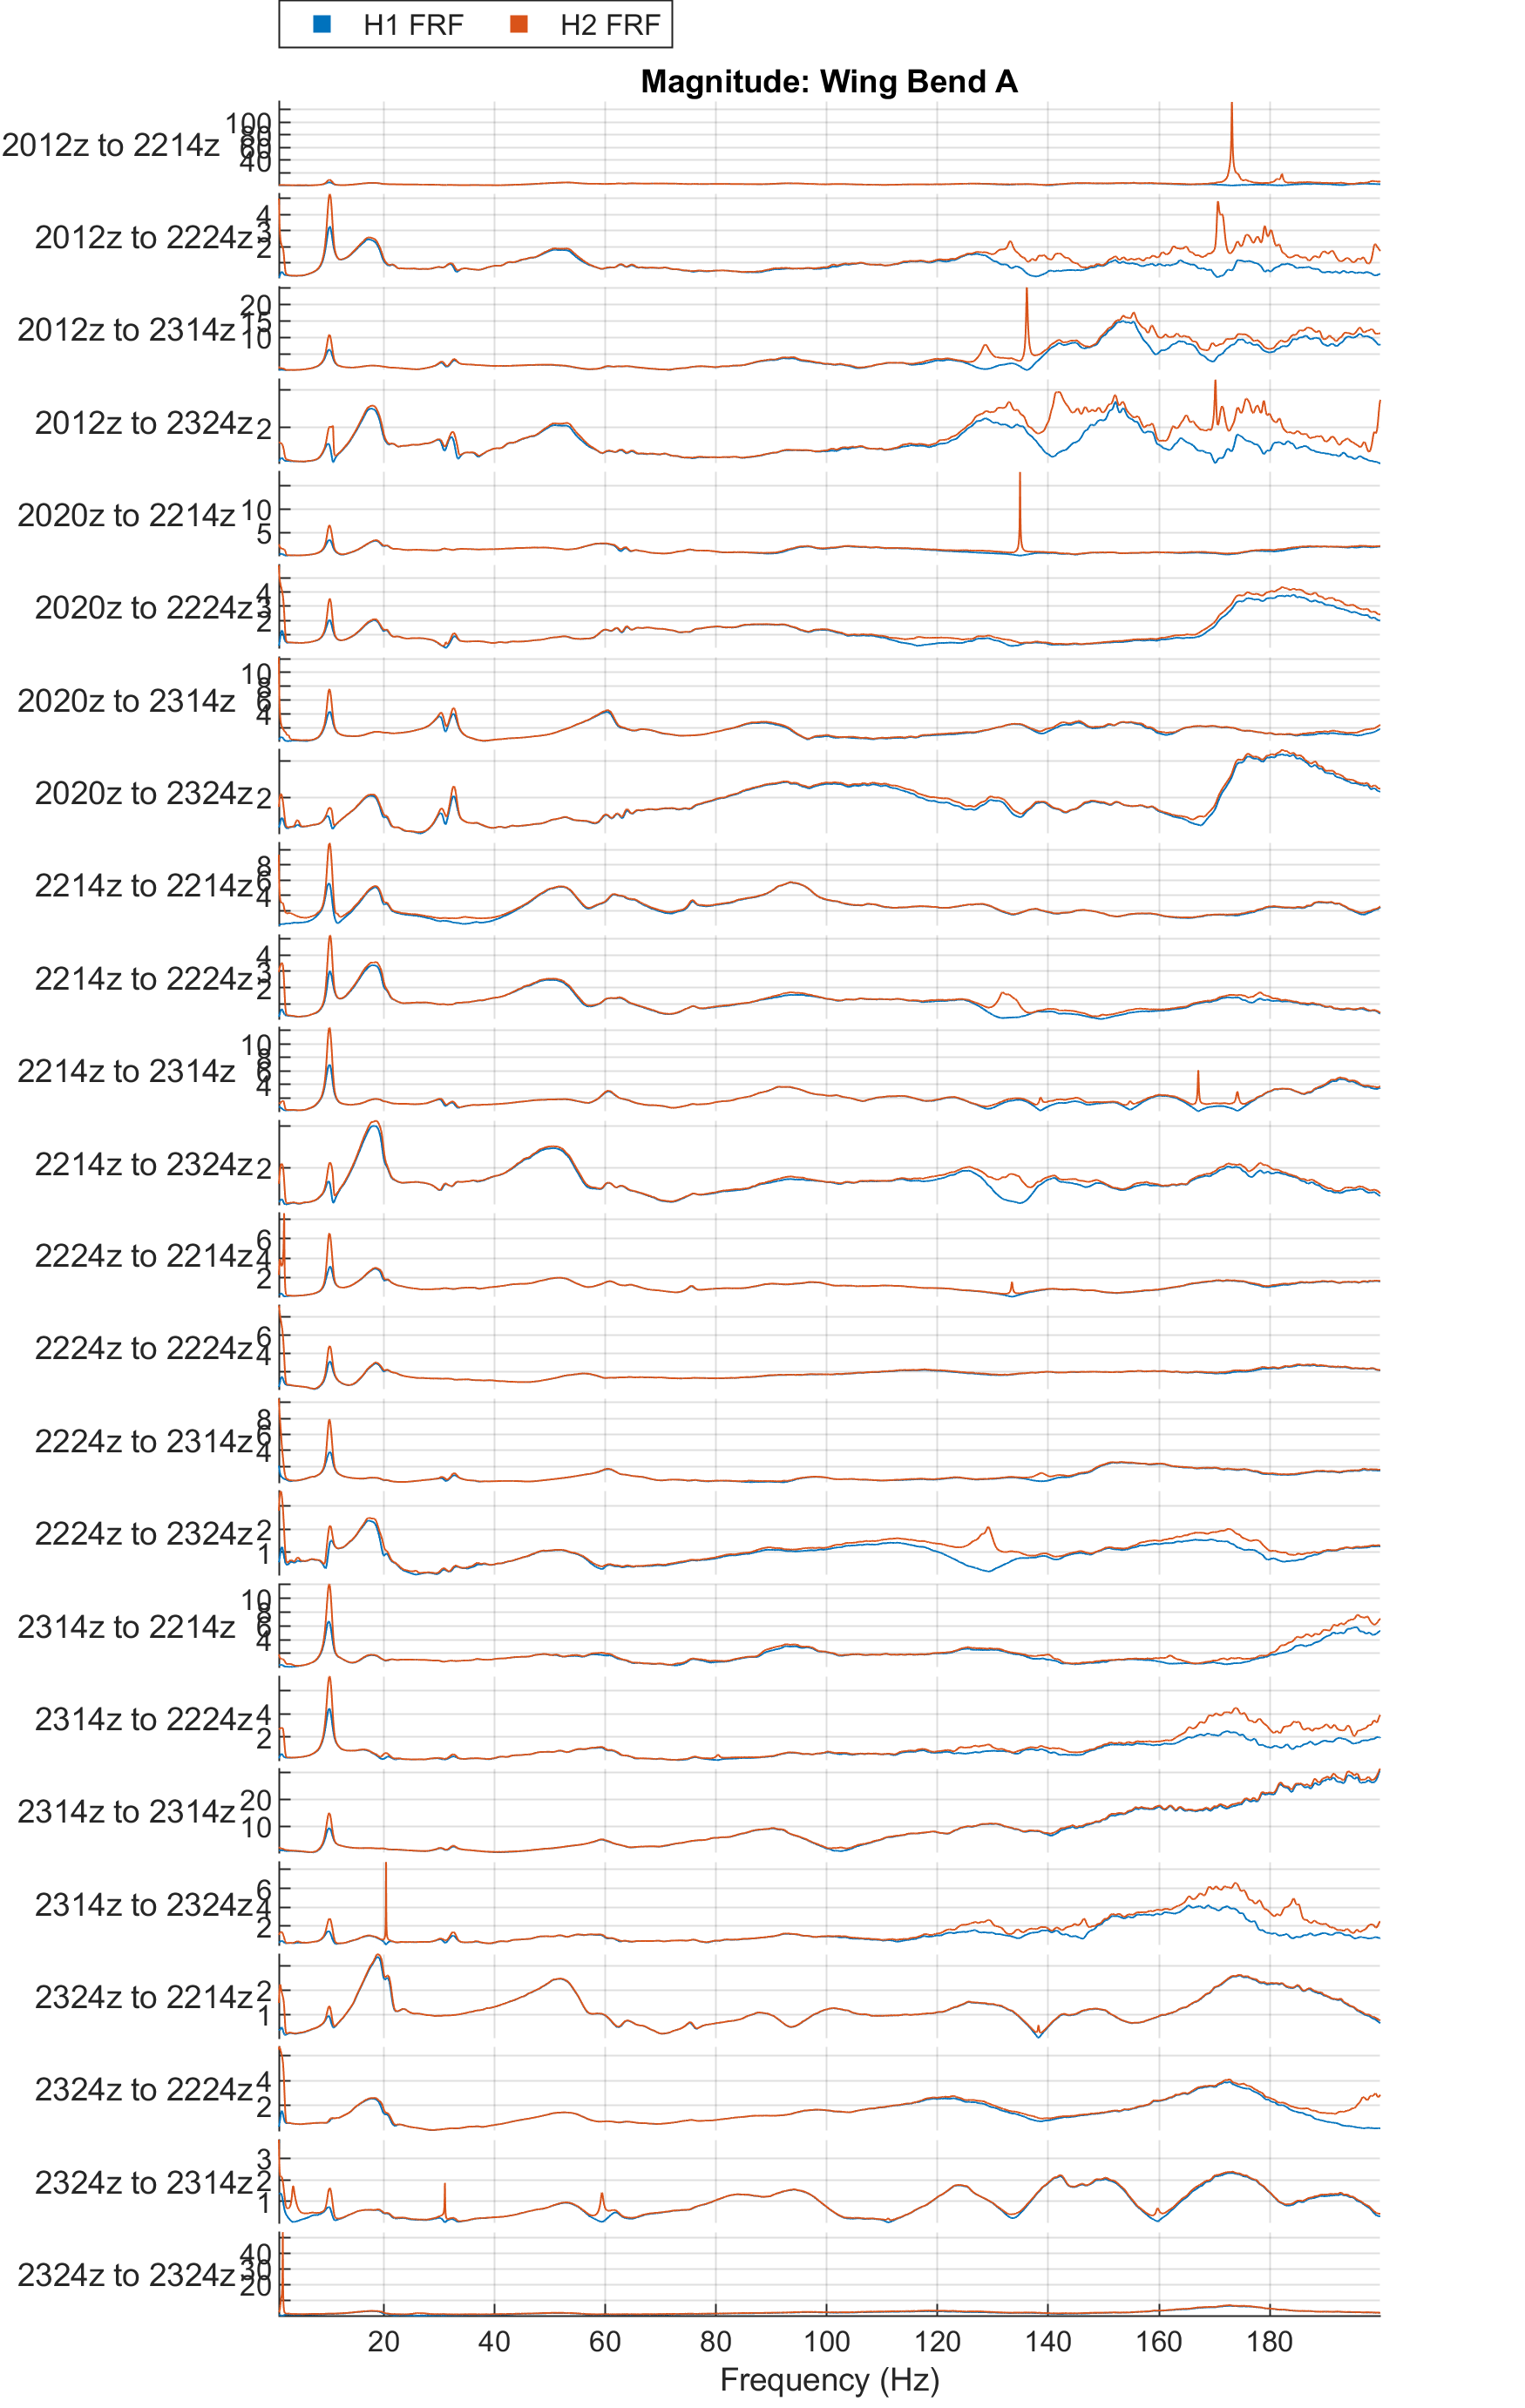
\includegraphics{figs/GVT/mag_Wing Bend A.png}
    \label{fig:mag_wingBendA}
\end{figure}
\begin{figure}[H]
    \centering
    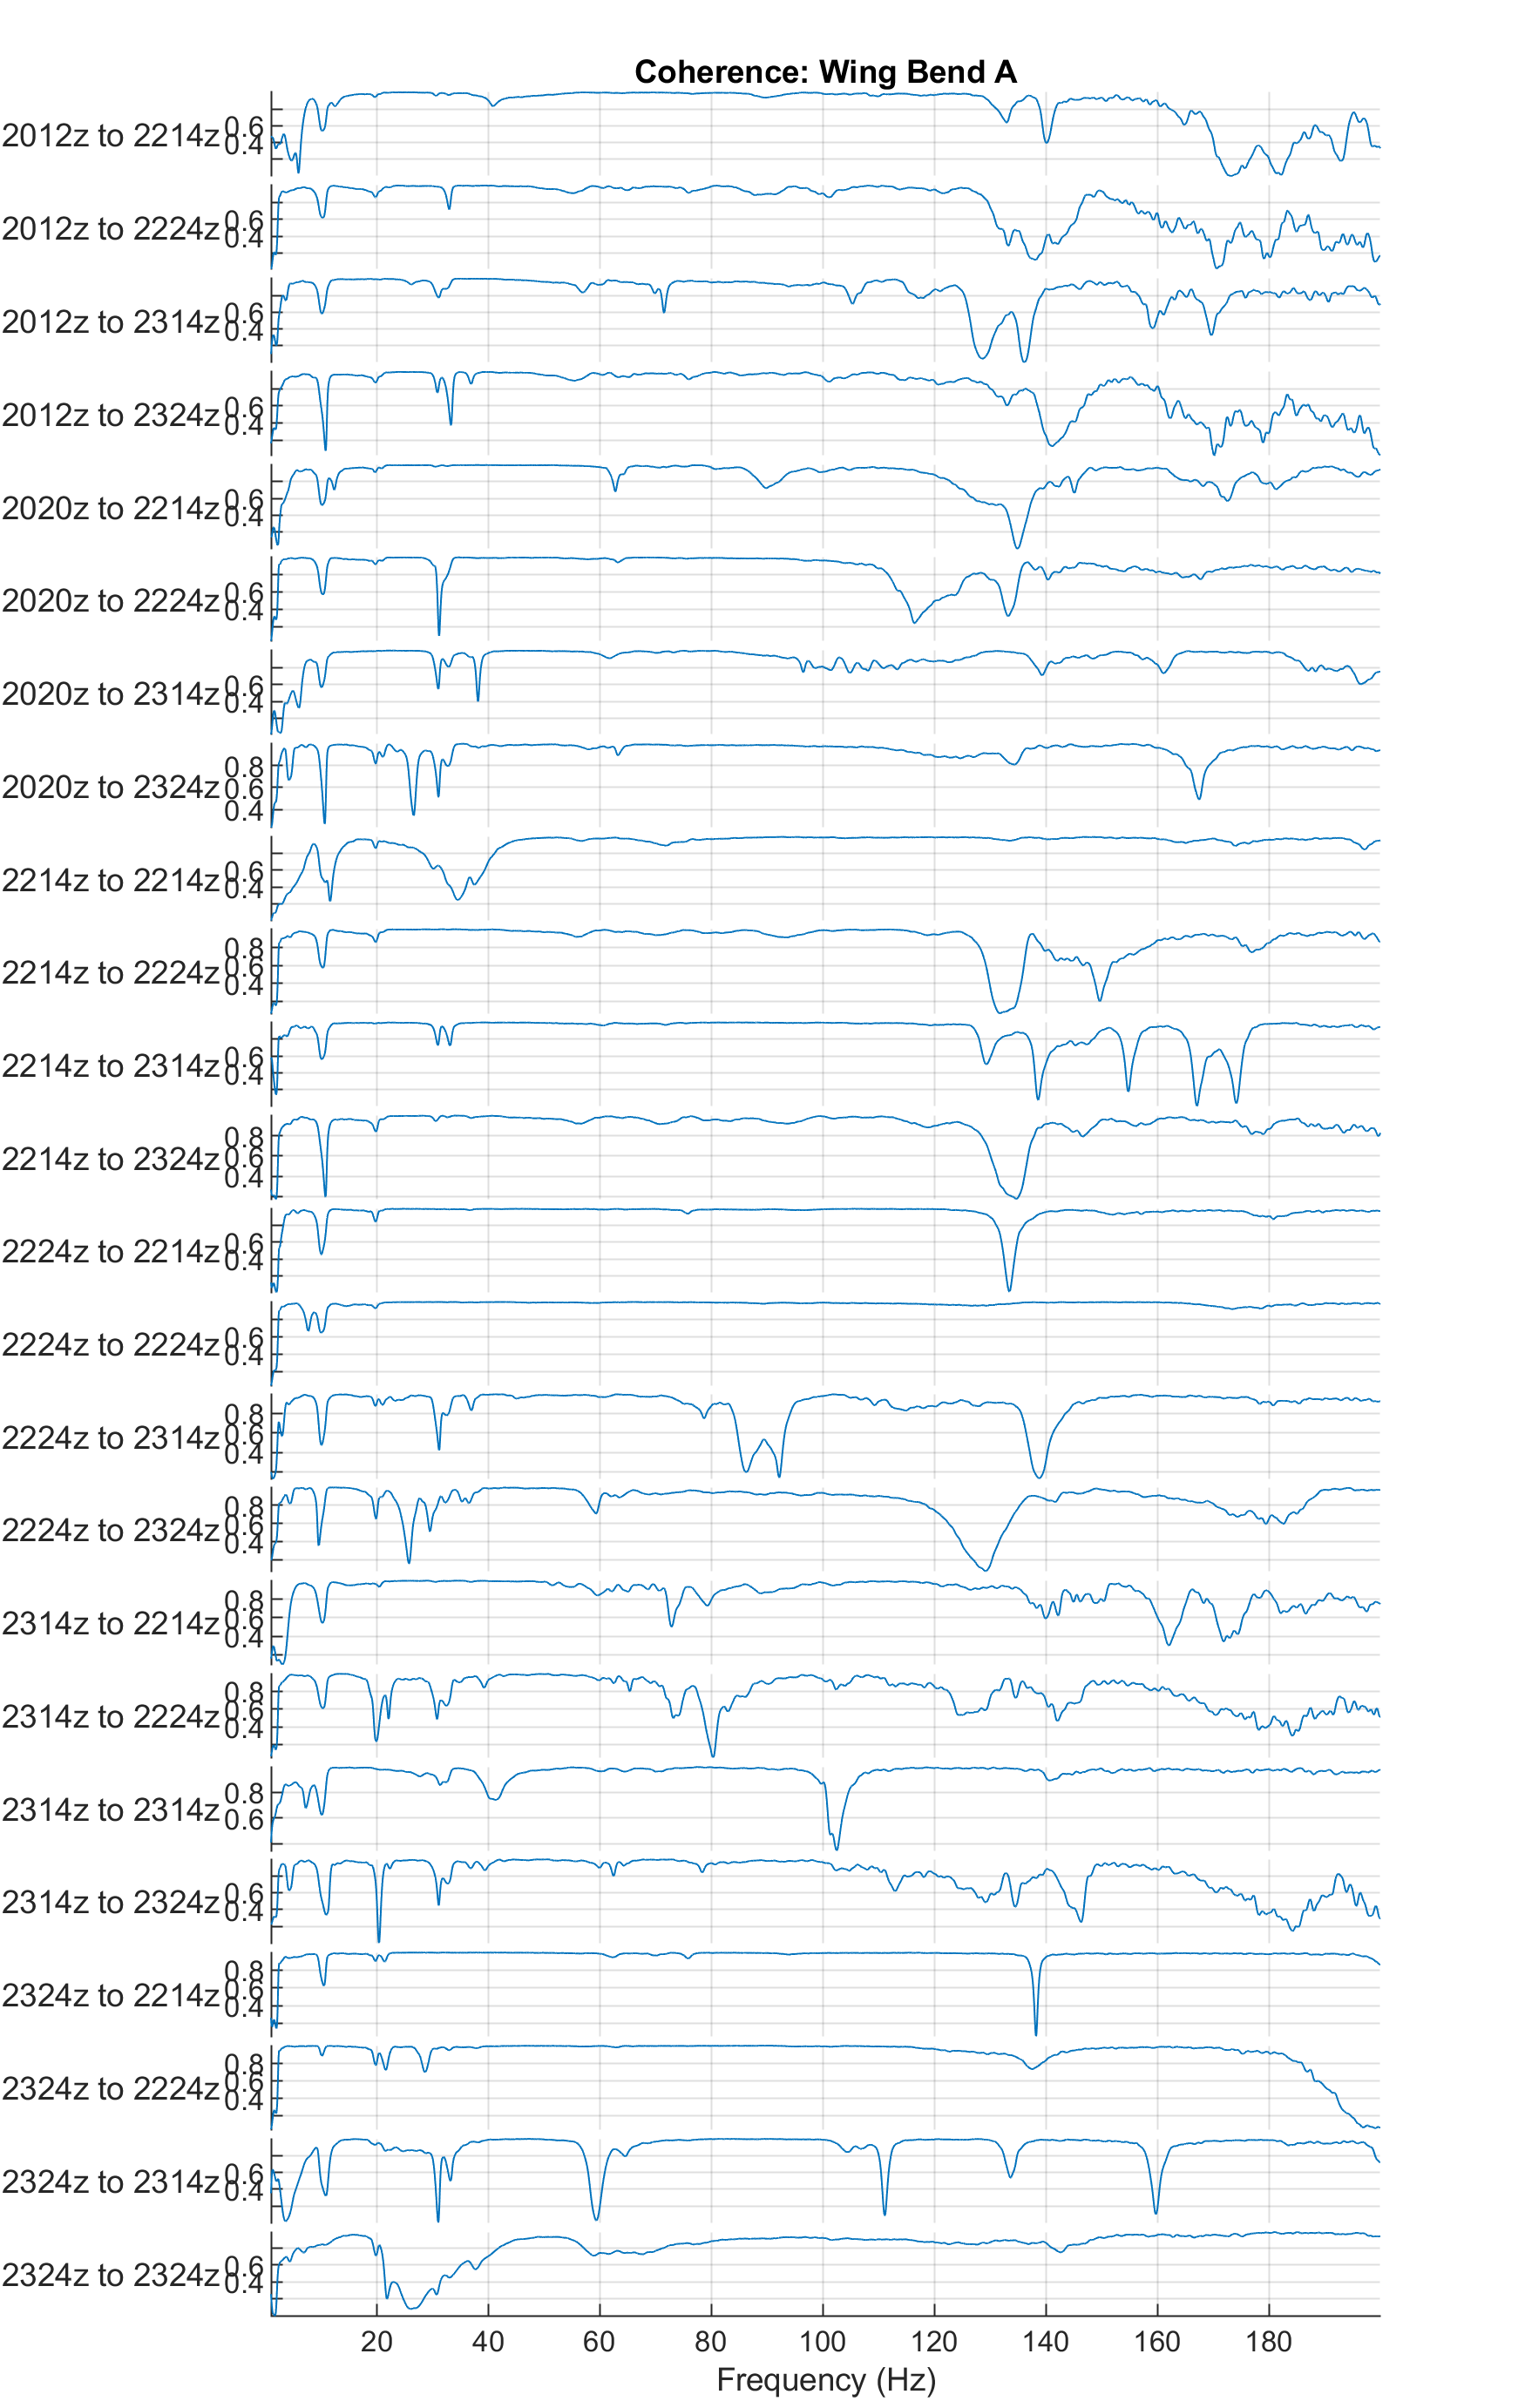
\includegraphics{figs/GVT/coh_Wing Bend A.png}
    \label{fig:coh_wingBendA}
\end{figure}

\begin{figure}[H]
    \centering
    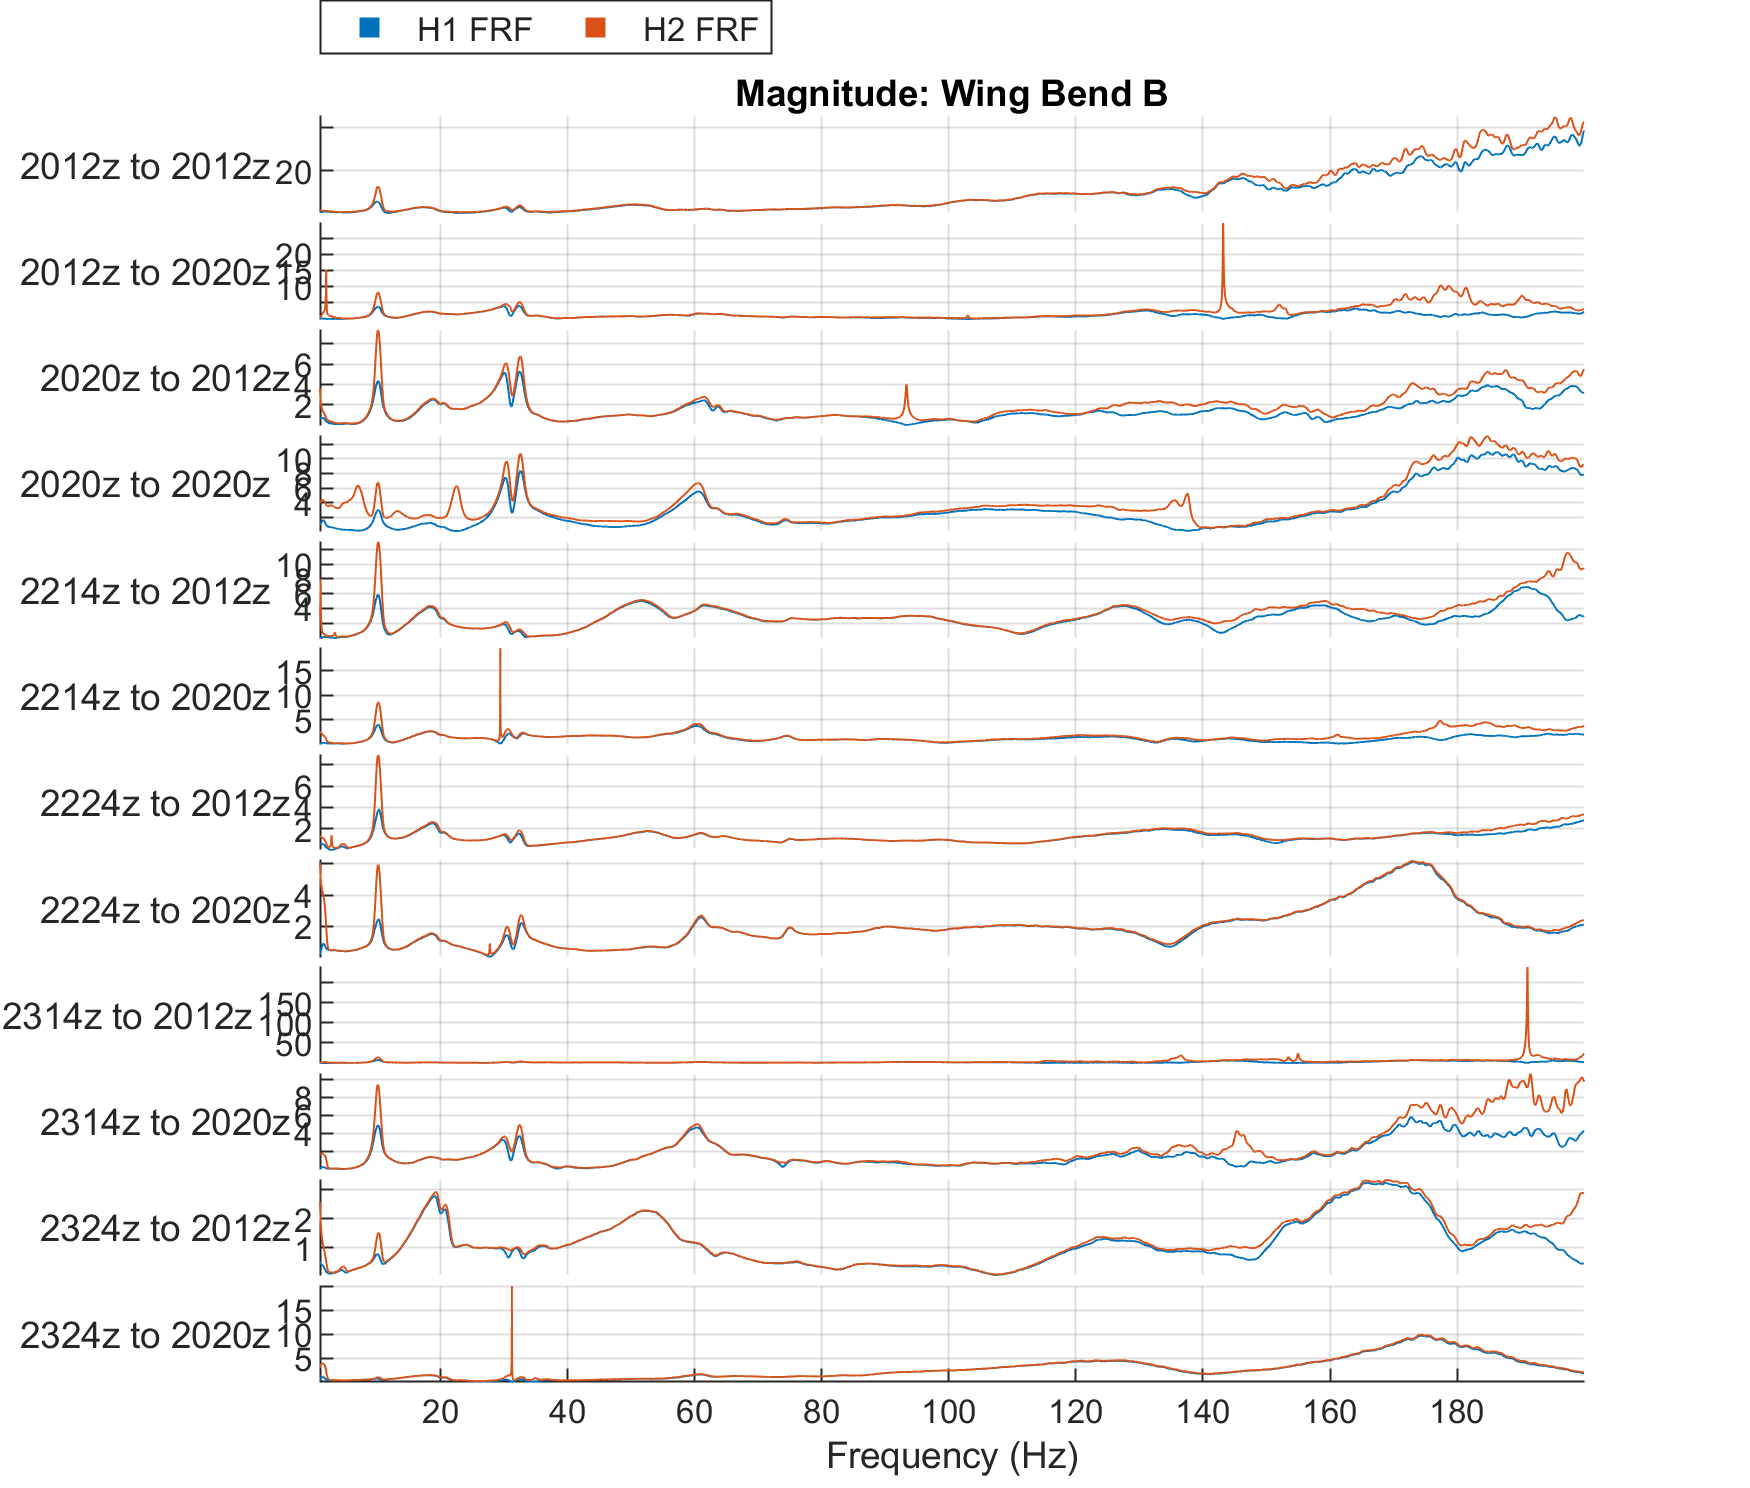
\includegraphics{figs/GVT/mag_Wing Bend B.png}
    \label{fig:mag_wingBendB}
\end{figure}
\begin{figure}[H]
    \centering
    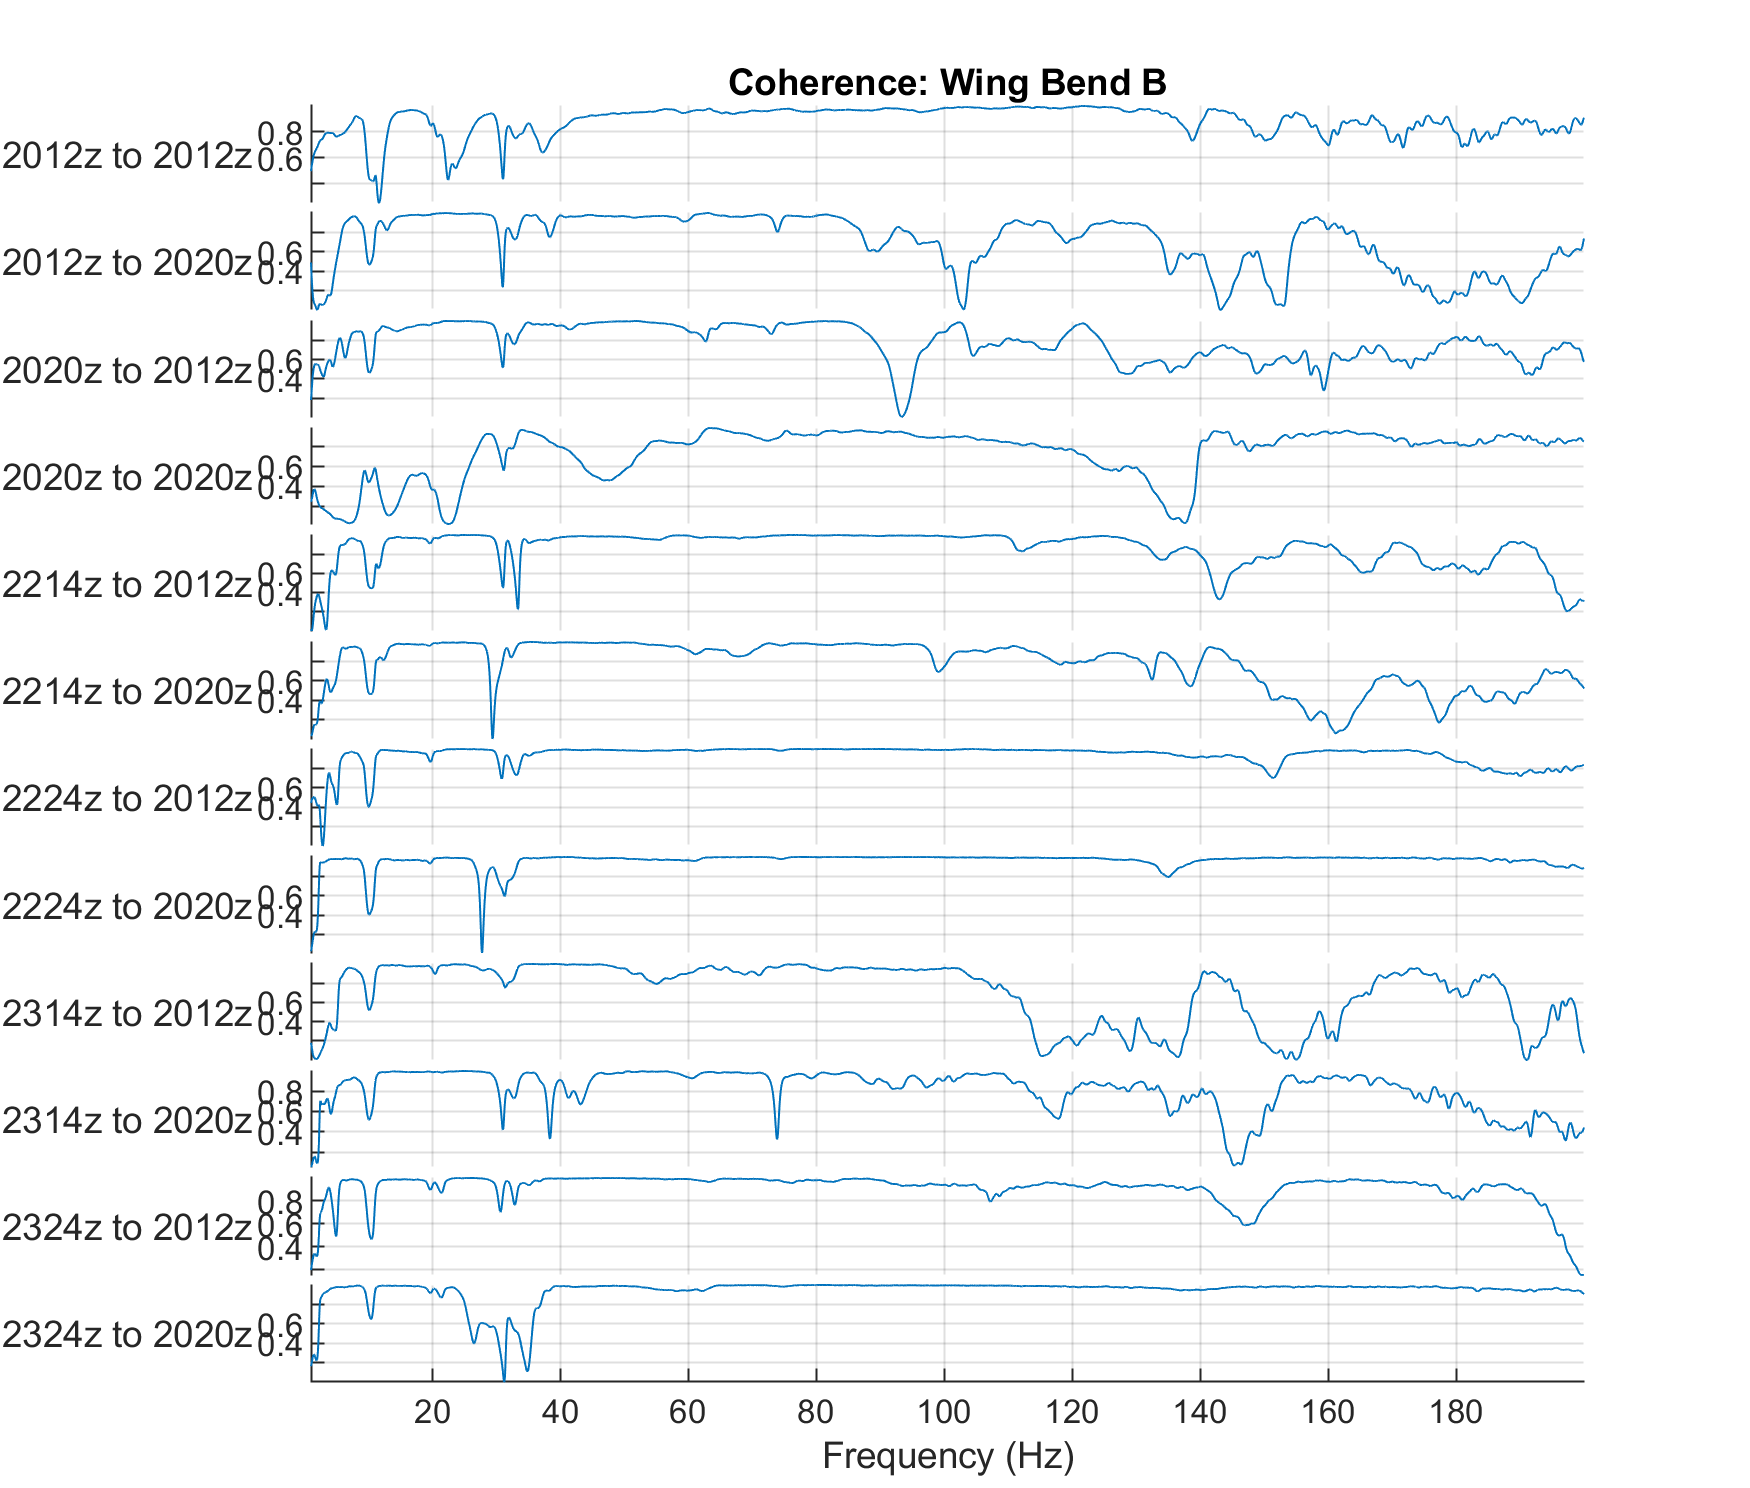
\includegraphics{figs/GVT/coh_Wing Bend B.png}
    \label{fig:coh_wingBendB}
\end{figure}

\begin{figure}[H]
    \centering
    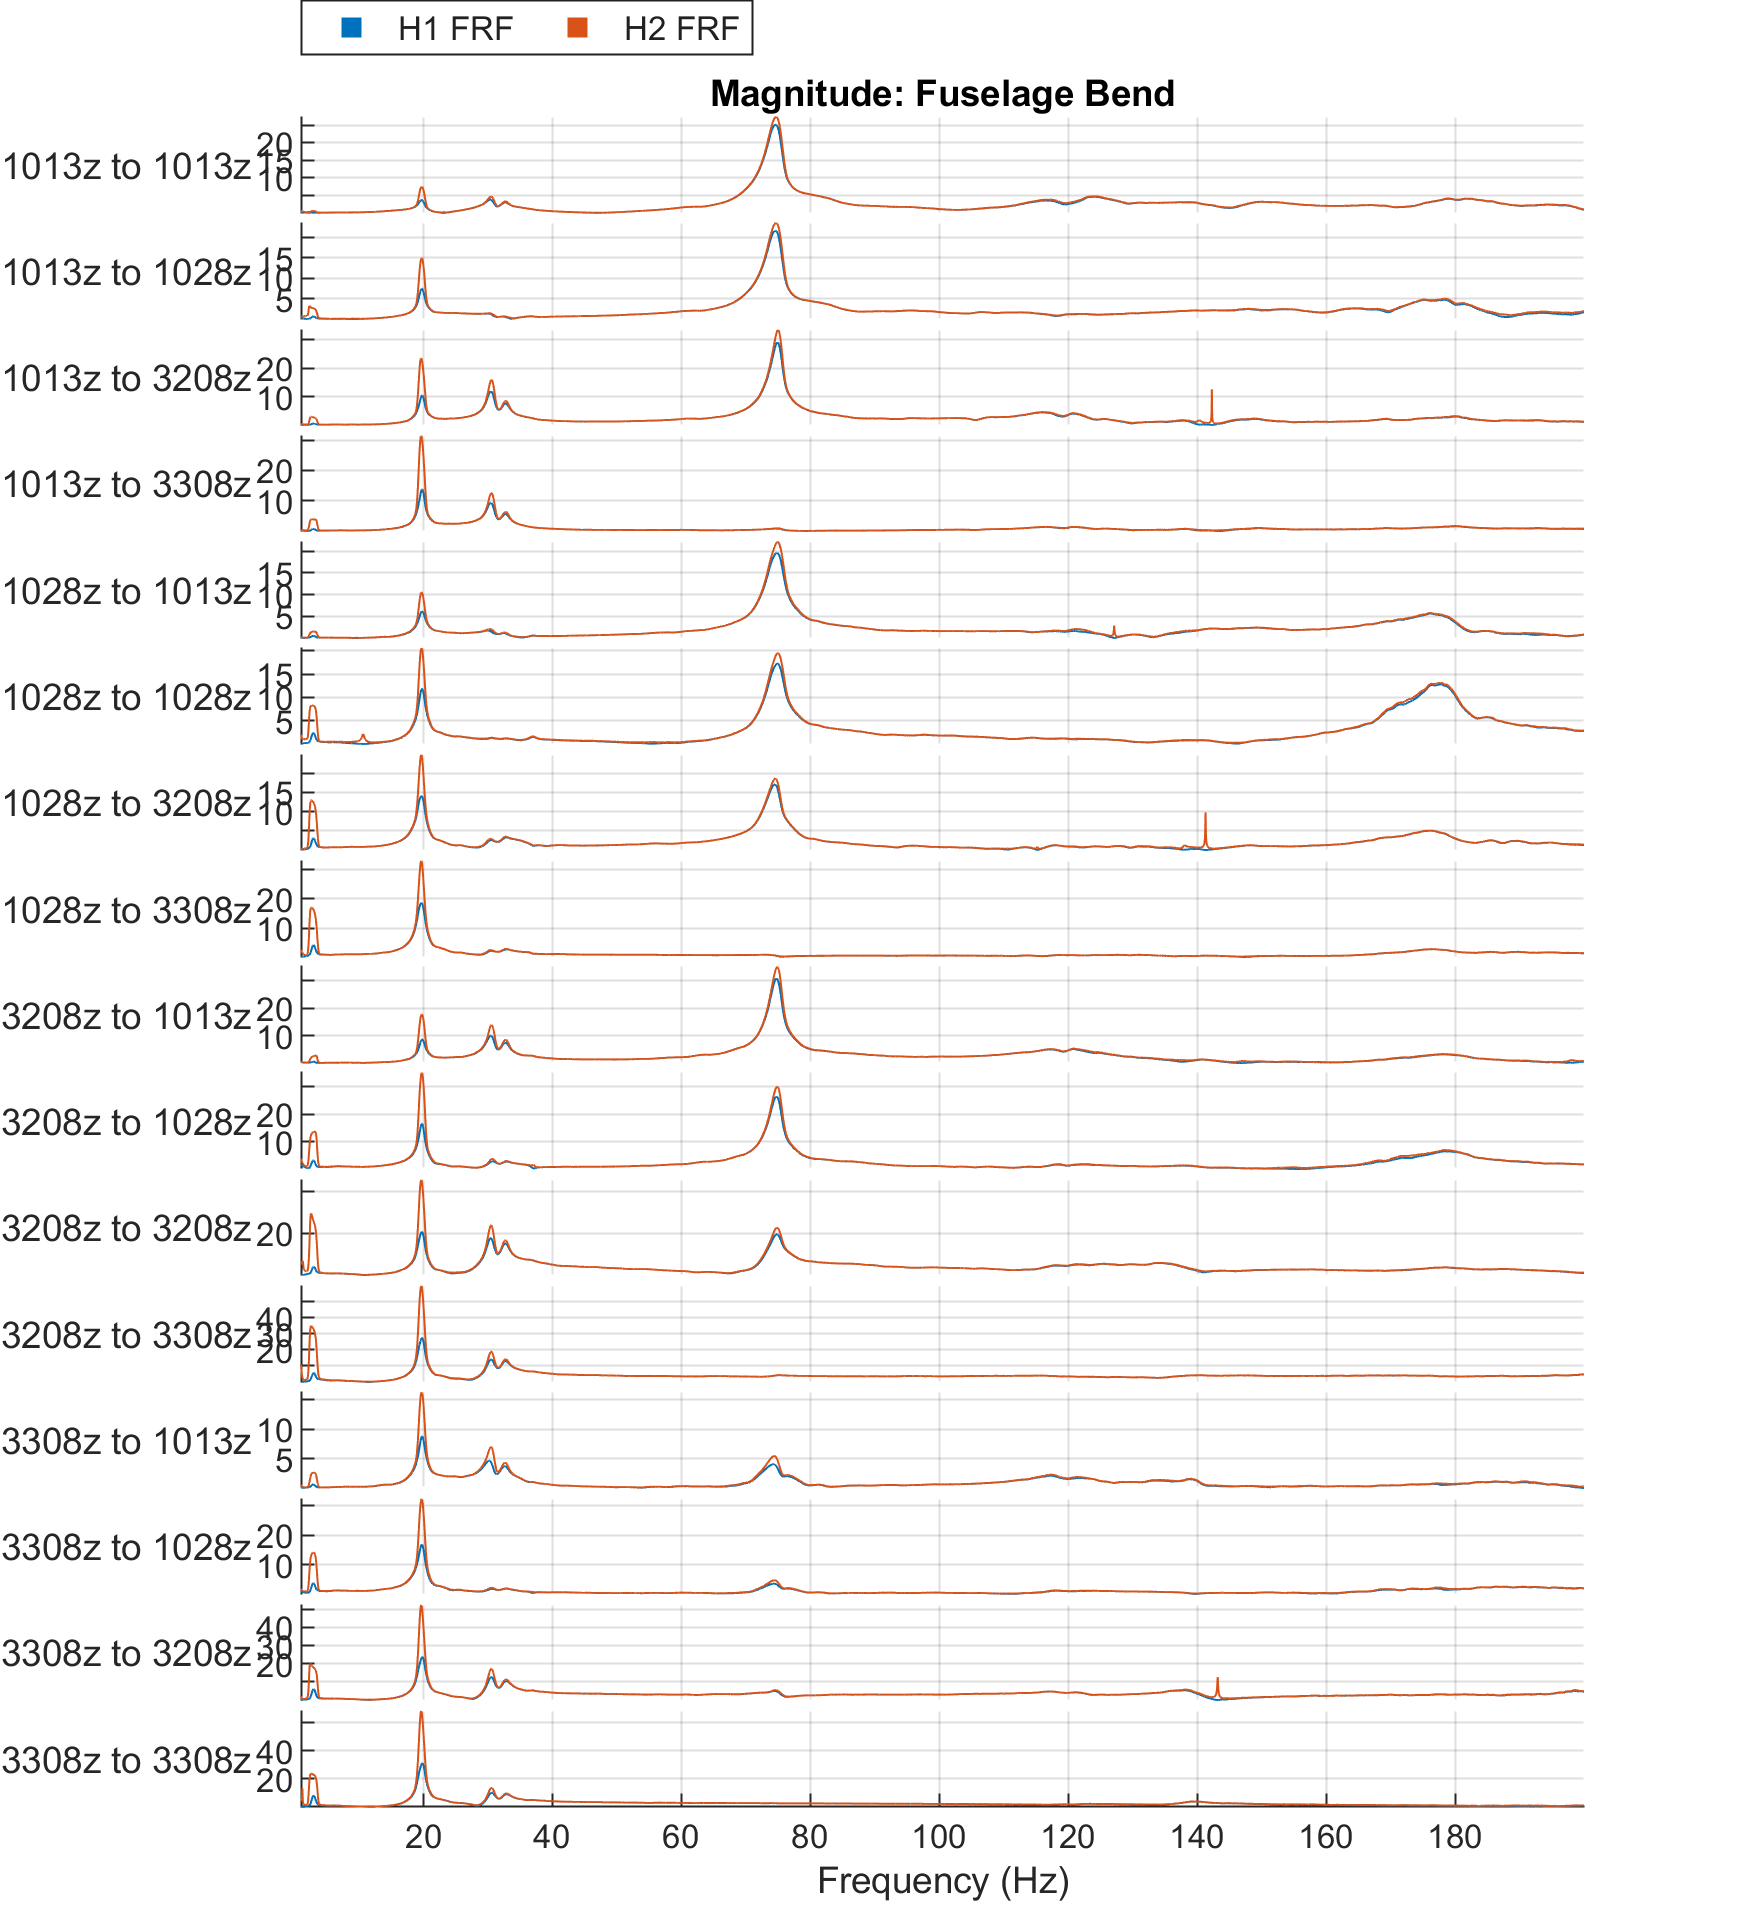
\includegraphics{figs/GVT/mag_Fuselage Bend.png}
    \label{fig:mag_fuseBend}
\end{figure}
\begin{figure}[H]
    \centering
    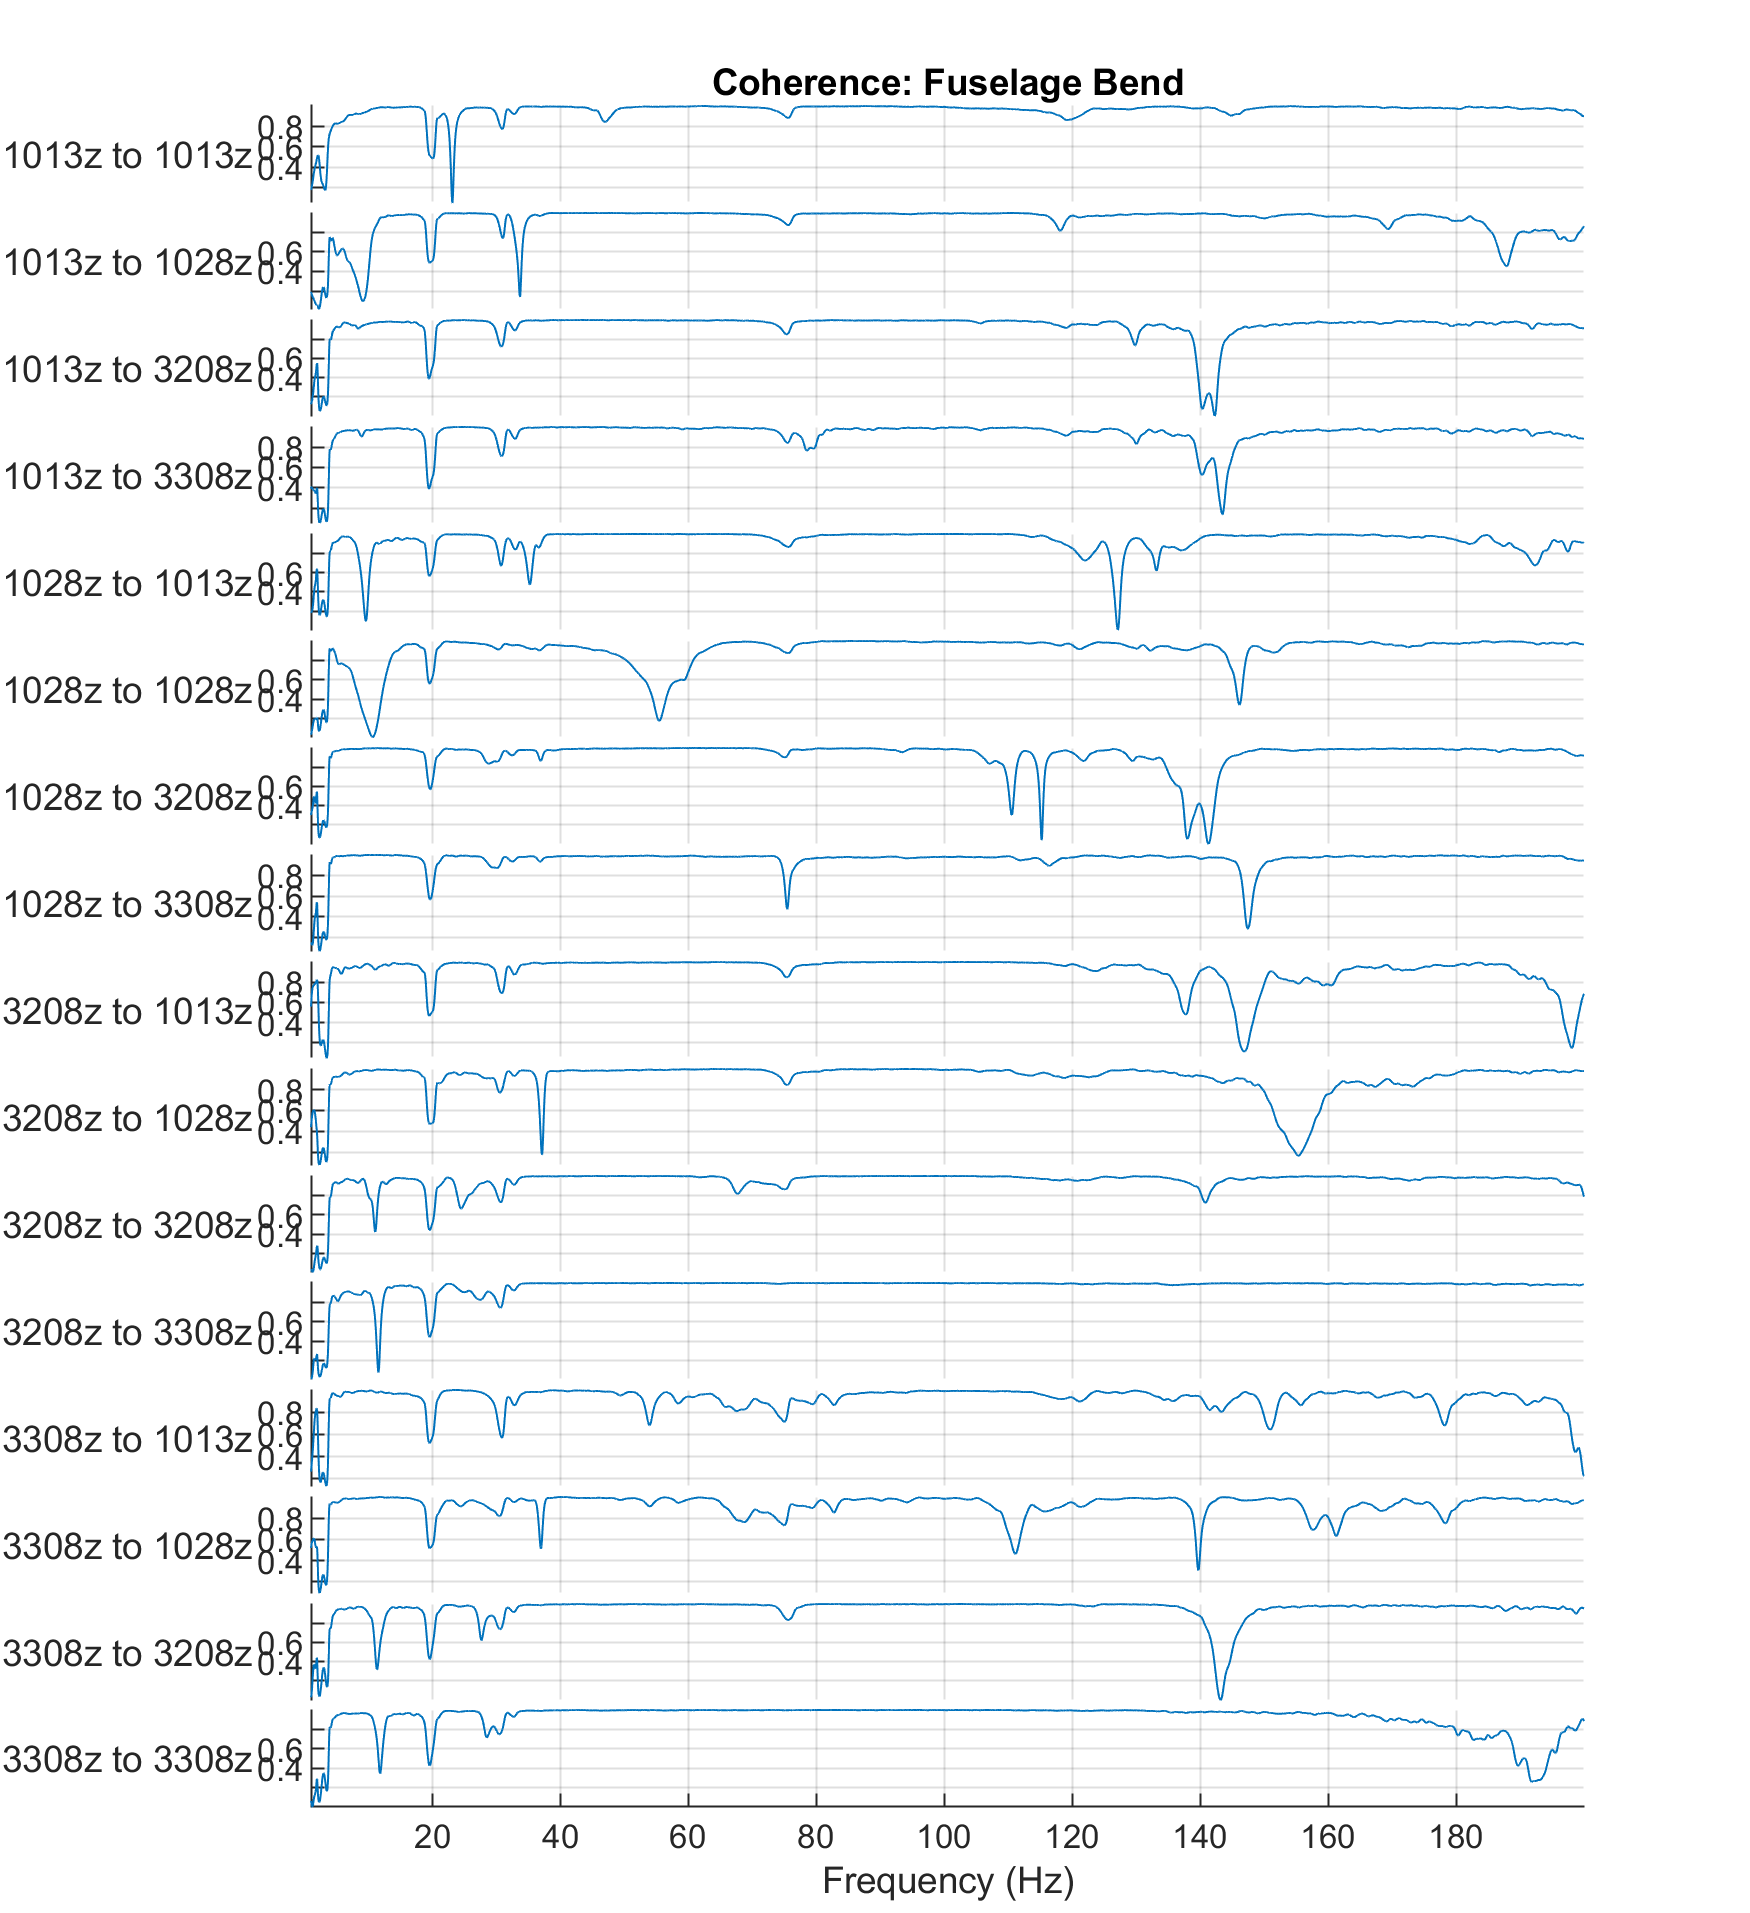
\includegraphics{figs/GVT/coh_Fuselage Bend.png}
    \label{fig:coh_fuseBend}
\end{figure}

\begin{figure}[H]
    \centering
    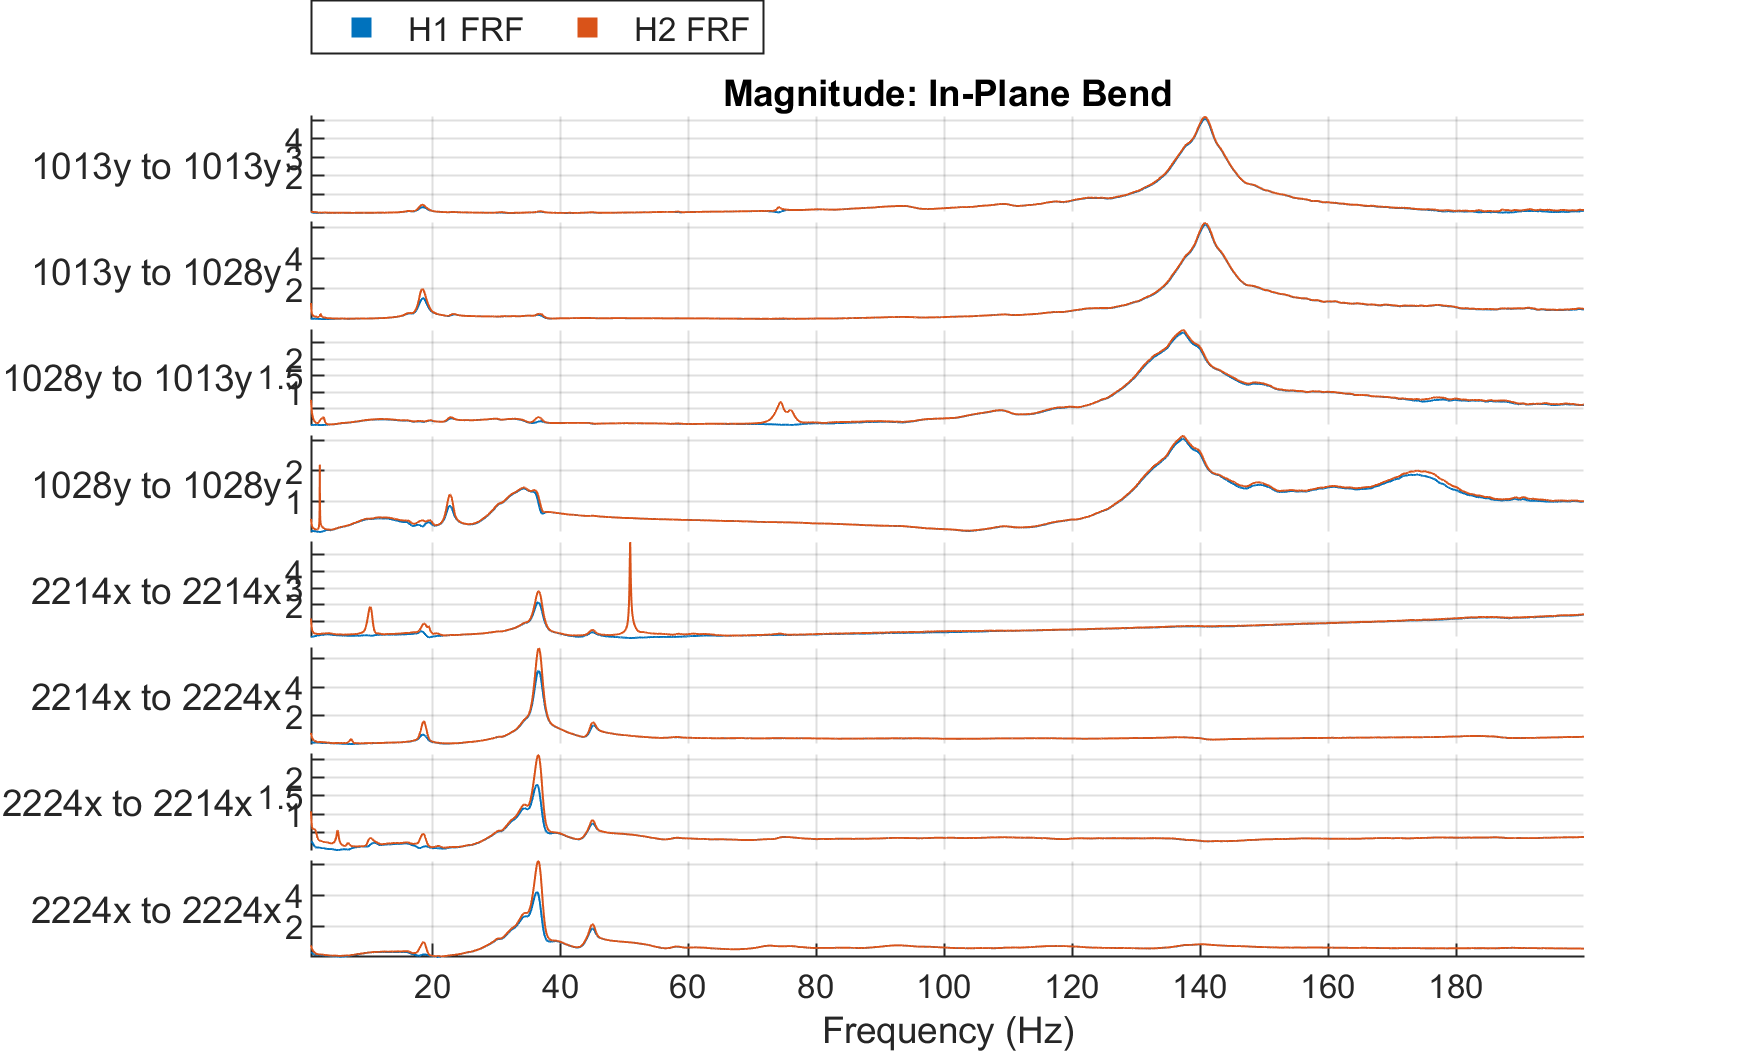
\includegraphics{figs/GVT/mag_In-Plane Bend.png}    
    \label{fig:mag_inPlaneBend}
\end{figure}
\begin{figure}[H]
    \centering
    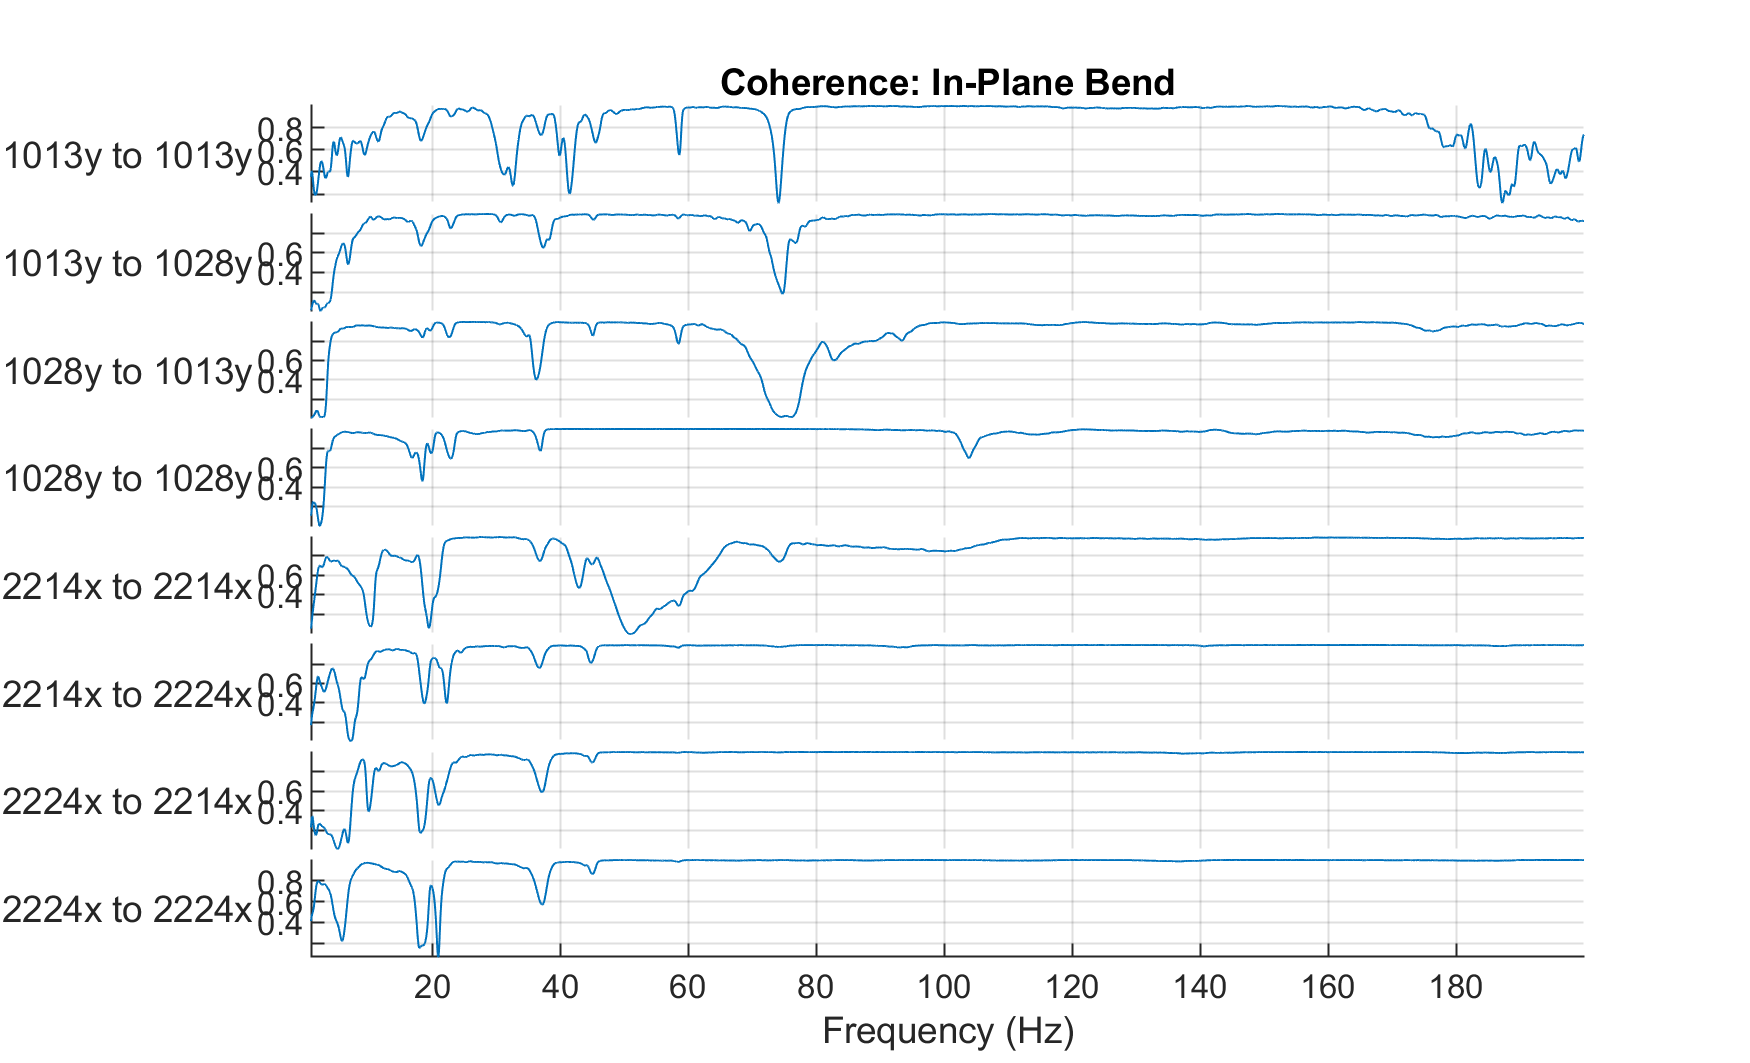
\includegraphics{figs/GVT/coh_In-Plane Bend.png}
    \label{fig:coh_inPlaneBend}
\end{figure}

\begin{figure}[H]
    \centering
    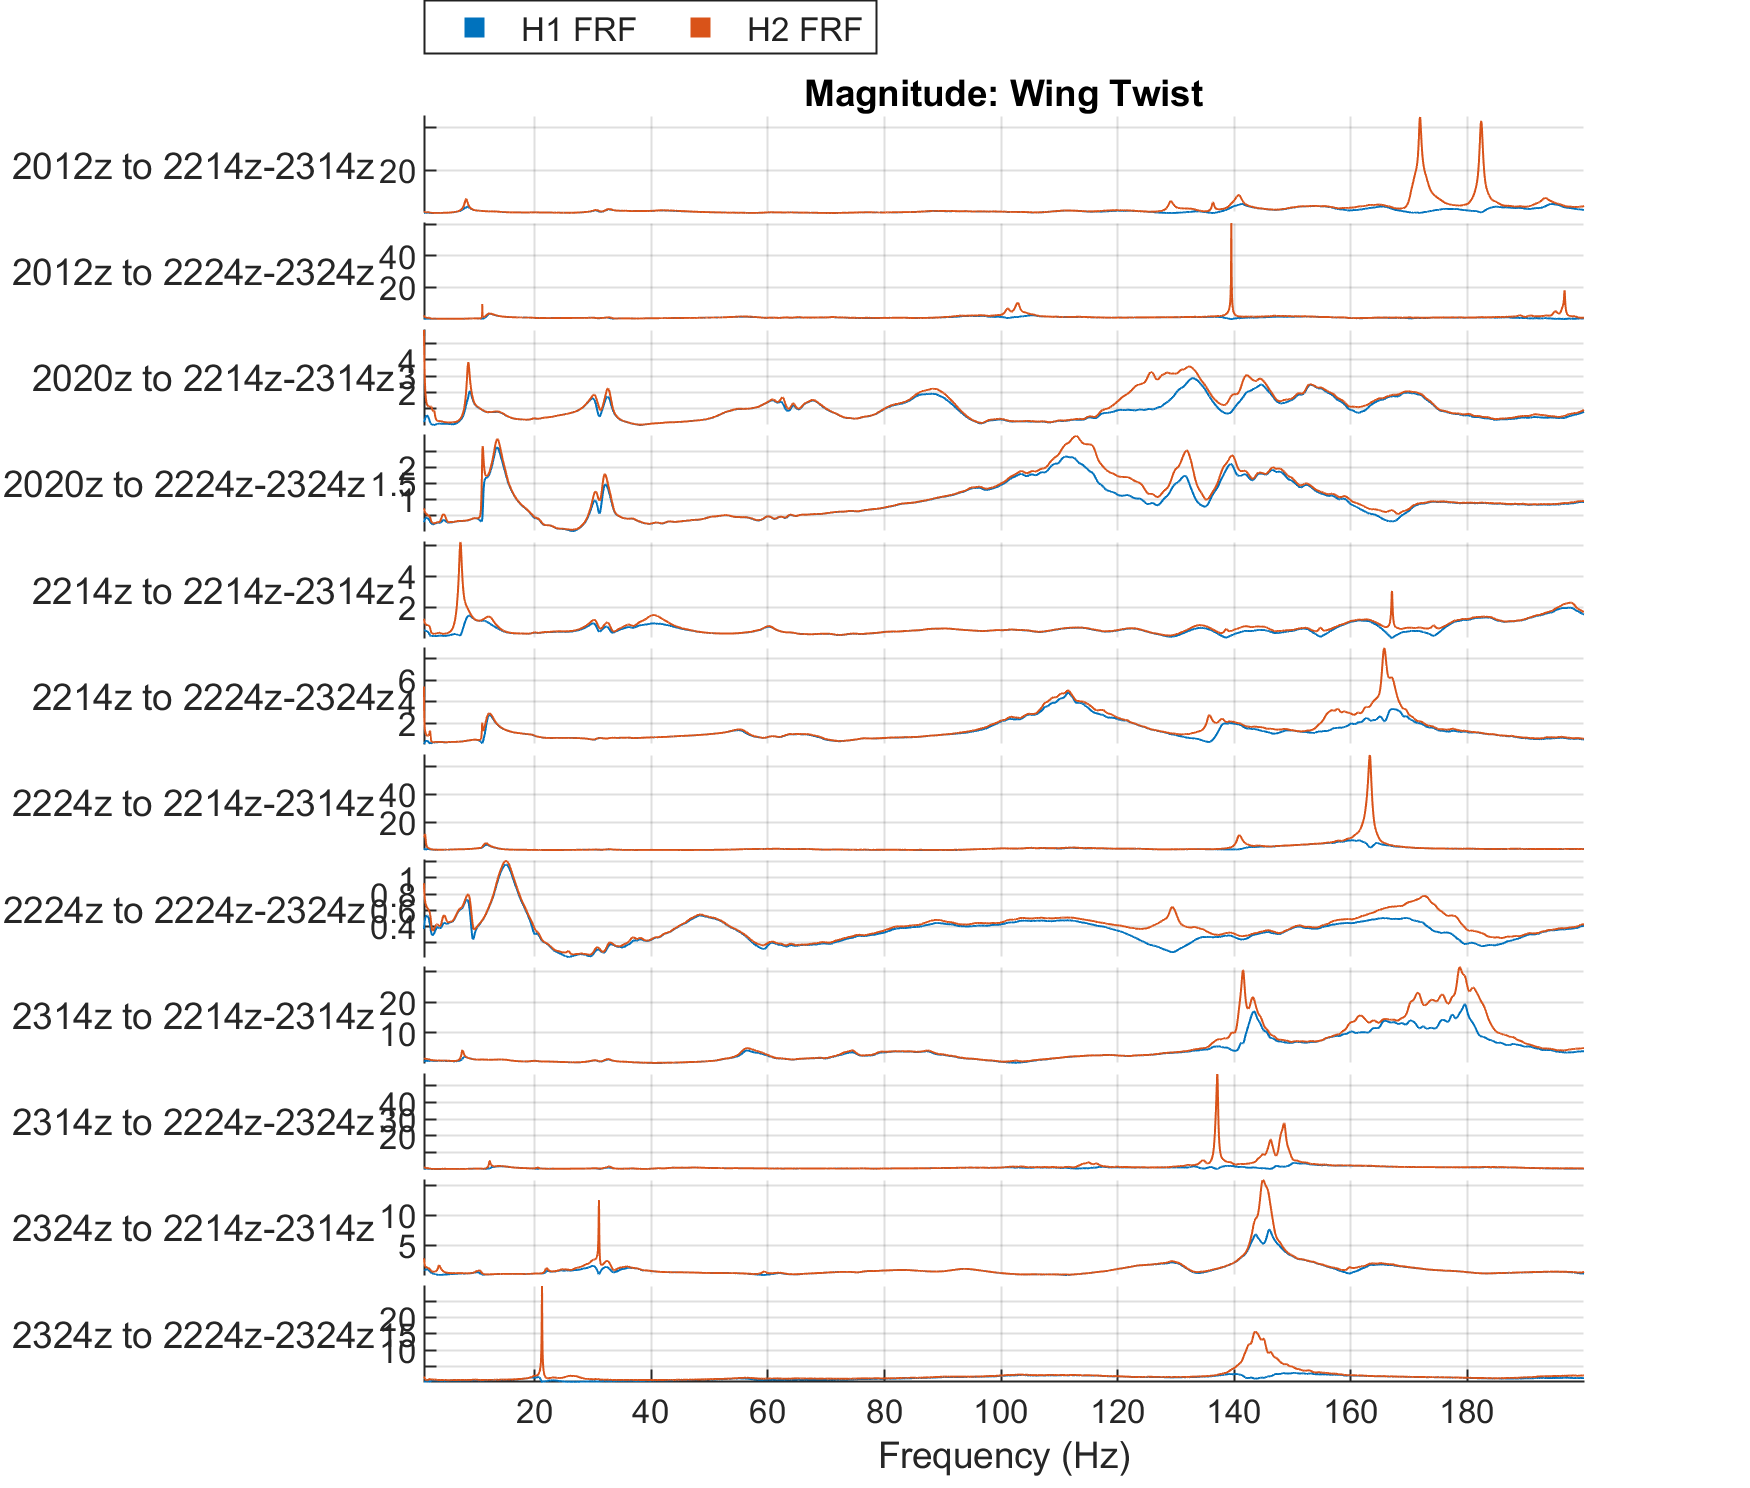
\includegraphics{figs/GVT/mag_Wing Twist.png}
    \label{fig:mag_wingTwist}
\end{figure}
\begin{figure}[H]
    \centering
    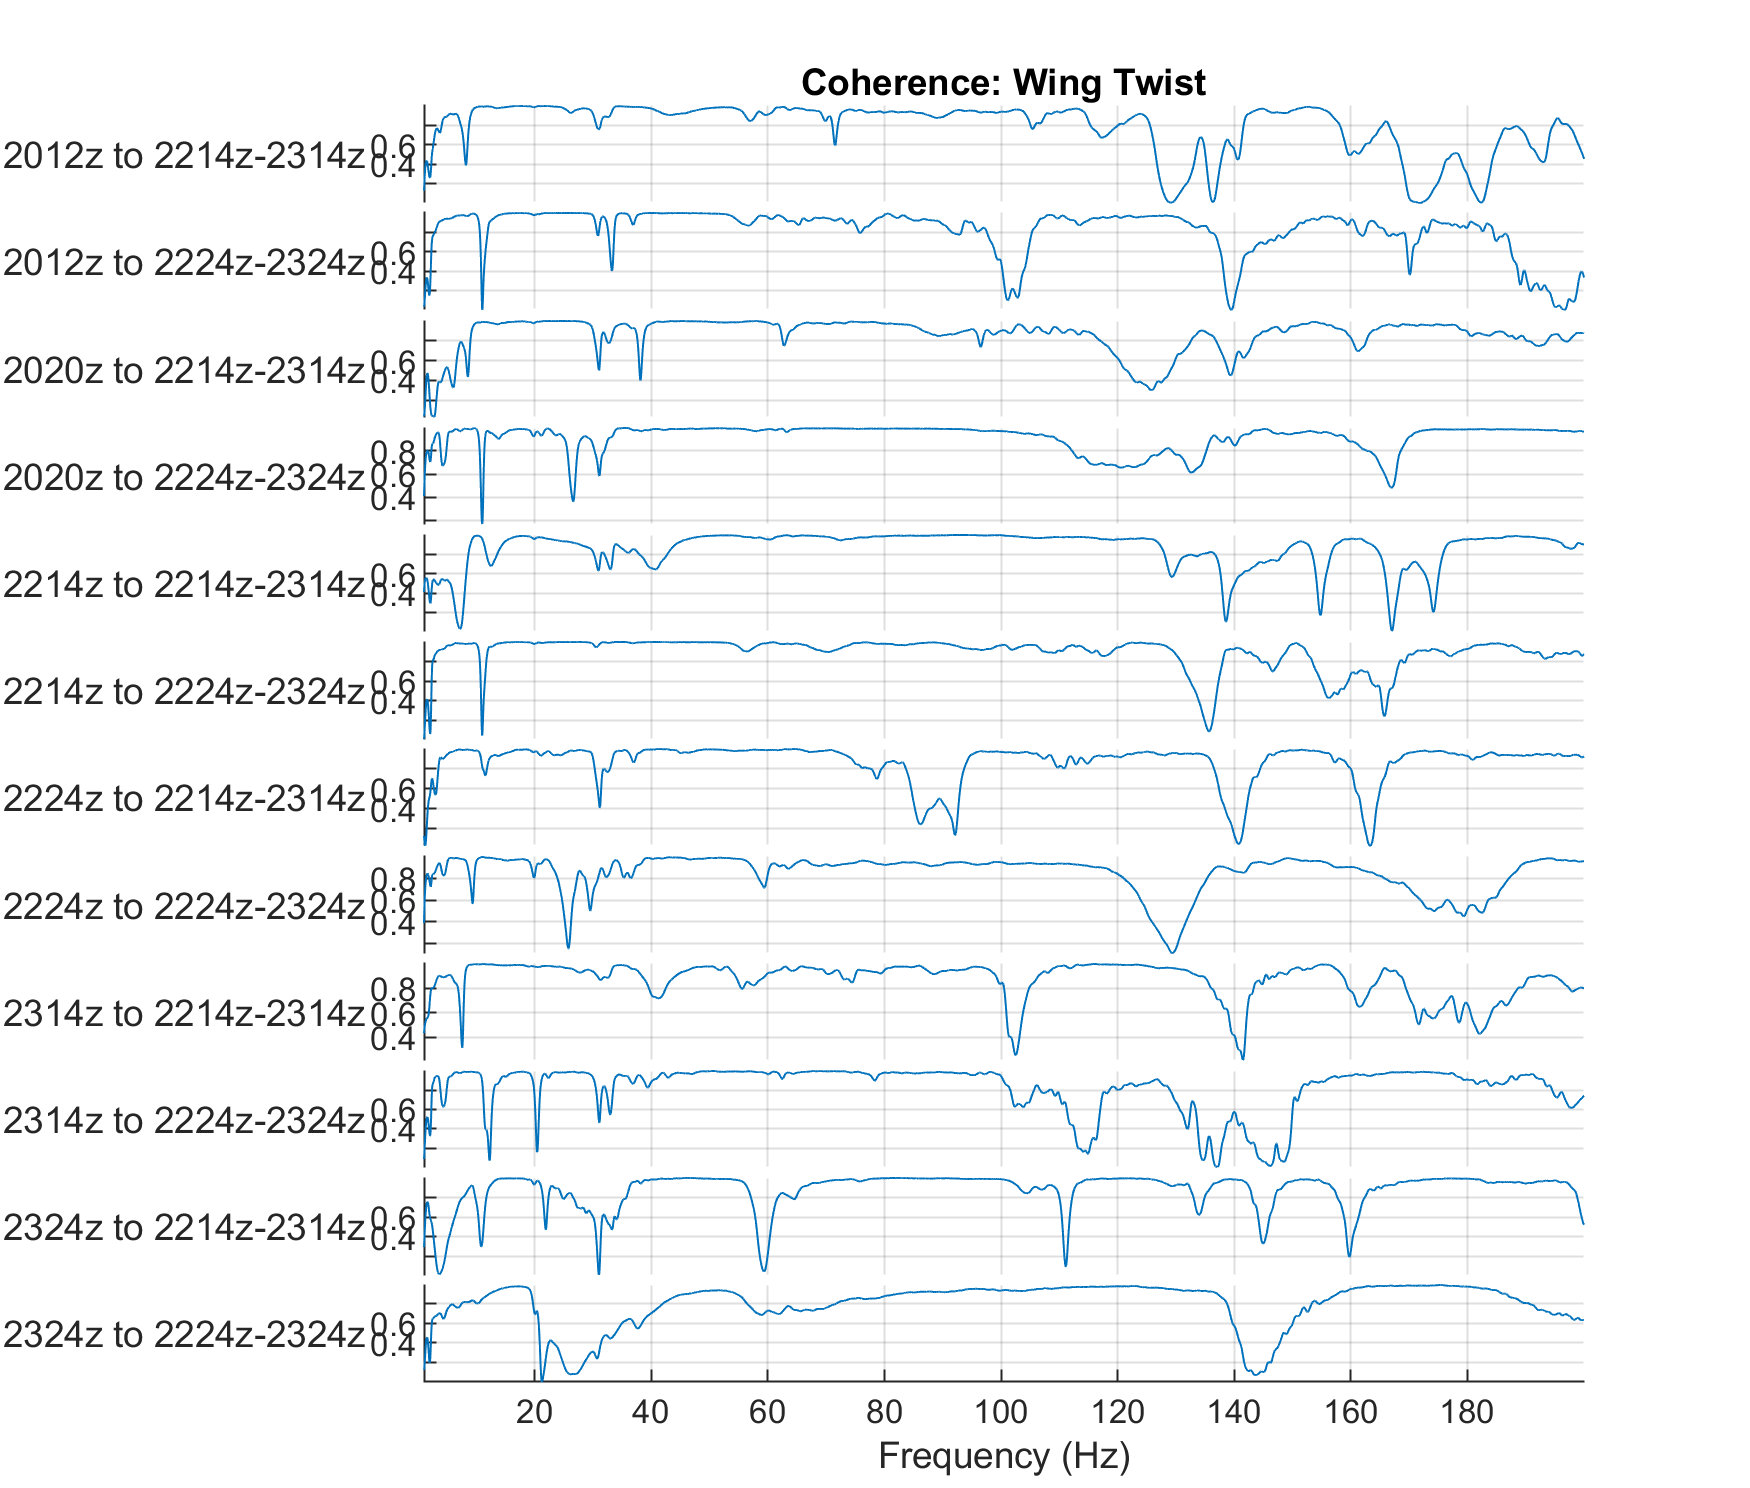
\includegraphics{figs/GVT/coh_Wing Twist.png} 
    \label{fig:coh_wingTwist}
\end{figure}